\scanpage{41}
\mspage{22}
of $\zeta',\zeta_1$ or of only one of these quantities
\[
(75)\qquad\begin{aligned}
\beta'&=\zeta_1\sigma_\infty(\zeta')^{-1}=\deleted{\varepsilon_0(\lambda\zeta_1)}\zeta_1(\sigma_\infty\varepsilon_0)(\lambda\zeta_1)^{-1}\\
&=\lambda^{-1}\cdot\varepsilon_0^{-1}(\zeta')\sigma_\infty(\zeta')^{-1}.
\end{aligned}
\]
from \deleted{the last} \inserted{these} expressions for $\beta'$ one obtains
\[
(75')\qquad\begin{aligned}
\sigma_\infty(\beta')&=\sigma_\infty(\zeta_1)\zeta'^{-1}=\sigma_\infty(\zeta_1)\varepsilon_0(\lambda\zeta_1)^{-1}\\
&=\sigma_\infty(\lambda)^{-1}\underbrace{\overbrace{\rho(\zeta')\zeta'^{-1}}^{\alpha'^{-1}}}_{\deleted{\unsure{\alpha'}}}
\end{aligned}
\]
and the third expression for $\beta'$ \deleted{gives}

\deleted{$(77)$ This said, the equation that $(72\,b)$ is equivalent to:}
\deleted{\[(77)\qquad\beta'\sigma_\infty(\beta')=1\]}
\deleted{that is, $\sigma_\infty(\beta')$ setting $\beta_1=\sigma_\infty(\beta')$, for}
\figure{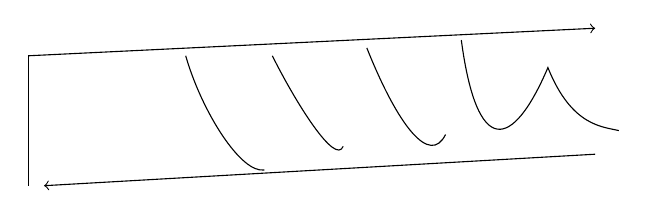
\begin{tikzpicture}[x=1cm,y=1cm]\draw[->] (0,1)--(7.2,1.35);\draw (0,1)--(0,-.65);\draw[->] (7.2,-.25)--(.2,-.65);\draw (2,1)..controls (2.2,.3) and (2.7,-.5)..(3,-.45);\draw (3.1,1)..controls (3.4,.4) and (3.9,-.4)..(4,-.15);\draw (4.3,1.1)..controls (4.7,.1) and (5.1,-.4)..(5.3,0);\draw (5.5,1.2)..controls (5.7,-.3) and (6.15,-.2)..(6.6,.85)..controls (6.9,.1) and (7.3,.1)..(7.5,.05);\end{tikzpicture}}
is also written
\[
(77)\qquad\sigma_\infty(\beta')^{-1}=\alpha'\sigma_\infty(\lambda).
\]
This being so, equation $(72\,b)$ is equivalent to
\[
(78)\qquad\beta'\sigma_\infty(\beta')=1\qquad\text{or again}\quad\sigma_\infty(\beta')^{-1}=\beta'
\]
which is invariant under the substitution $\beta'\mapsto\sigma_\infty(\beta')$ \unsure{or|\deleted{in}} $\beta'\mapsto\beta'^{-1}$, thus setting
\inserted{(without assuming $(*)$ to be satisfied)}
\[
\beta_1=\sigma_\infty(\beta')^{-1}=\alpha'\sigma_\infty(\lambda)
\]
equation (78) is equivalent to the equation
\[
(**)\qquad\beta_1\sigma_\infty(\beta_1)=1
\]
and implies that $\beta_1=\sigma_\infty(\beta_1)^{-1}$ hence $\beta_1=\beta'$.

In summary, one can immediately set
\[
(79)\qquad\beta'=\alpha'\sigma_\infty(\lambda)\qquad\text{where}\quad\alpha'=\zeta'\rho(\zeta')^{-1}
\]
and the relation to impose on $(\lambda,\zeta')$ is, at one's choice,
\margin{40}
